%************************************************
\chapter{HMRF clustering in the brain of \platyfull{}}\label{ch:biology} 
%************************************************


	\section{Choosing K with the BIC on biological data}
	After validating the HMRF method using simulated data as detailed in Chapter \ref{ch:simulations}, I now present the clustering results when the method is applied to the single cell expression dataset generated from the brain of \platy{}. Before interpreting the biological meaning of the inferred clusters, the first step is to choose $K$. To this end, as presented in Chapter \ref{ch:HMRF} I applied the BIC method.\\
	
	However, as shown in Figure \ref{fig:realBIC} (grey dots), the BIC does not reach a clear minimum but instead reaches a plateau after a given number of clusters. This is most likely due to the highly, but not perfectly symmetrical nature of the brain: with a small $K$, the same ``tissue" on both the left and the right hand side of the brain will belong to the same cluster. However, because the two sides of the brain are not perfectly symmetrical, as $K$ increases the left and right part of the same ``tissue" will be clustered separately. As a result, the likelihood continues to increase sufficiently to explain the flattened BIC curve.\\
	
	 Moreover, this hypothesis seems to be confirmed by the fact that when computing the BIC on the right and left side of the brain separately, the curve has in both cases a clear minimum as shown in Figure \ref{fig:realBIC} (red and green dots). Given this, I opted to choose $K$ as the point where the BIC curve reaches a plateau, that is when the derivative of the BIC curve become 0. I chose the start of the plateau stage if the BIC because, assuming the symmetry issue explained before, the BIC will reach a stable value when the cells on both sides of the brain are classified in the optimal number of clusters while conserving the left/right symmetry of the brain. \emph{Consequently for the rest of the Chapter, I considered the clusters identified for $K = 33$.} Importantly, the BIC starts to rise after $K=66$, which seems to confirm, assuming the symmetry hypothesis described above, that $K=33$ is a sensible choice. \\
	 
	 
	
	\begin{figure}[h]
\centerline{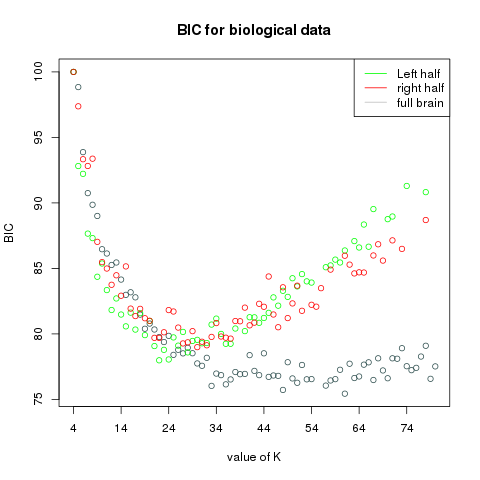
\includegraphics[width=\linewidth]{gfx/chapter6/real_BIC.png}}
\caption{{\bf BIC results on biological data.} Results are shown for $K \in [4,80]$ (x axis) with the full brain, and for the left and right half separately. The y axis shows the BIC value as a \% of the highest BIC value for each dataset.}
\label{fig:realBIC}
	\end{figure} 
	
	
	The main output of the method is a list of $S=32.203$ cluster assignments, that is, the cluster each ``cube'' of the in-situ hybridization data belongs to. With this output and the spatial coordinates of each cube, it is easy to use the bioWeb3D tool presented in Chapter \ref{ch:non_spatial_clustering_visualization} to visualize the clusters in the brain. However, downstream analysis solely based on the spatial localization of the clusters is insufficient, and it is possible to take advantage of the model's output parameter values to analyse and interpret the biological meaning of the resulting clusters.

	\section{Parameters interpretation}
	The parameter $\Theta$ can be used to shed light on the biological meaning of the inferred clusters. As described in the previous chapters, for $h \in K$ and $m \in M$, $\hat{\theta_{h,m}}$ is the probability that gene $m$ is expressed in a given cell contained in cluster $h$. Therefore, the values of $\Theta$ provide a link between the mathematical model and downstream biological interpretation.\\
	
	However, in practice, not all of the 86 genes will provide insight into the biological function of a given cluster. For instance, in the case of a ubiquitously expressed gene, $g$, the value of $\boldsymbol{\theta_{h,g}}$ will be high for all clusters. To overcome this problem, I developed a score, $S$, for each gene, $m$ and each cluster $h$, where:
\begin{align*}
s_{hm} = \frac{\theta_{h,m}}{\sum_{a} \theta_{a,m}}.
\end{align*}

For each gene, $m$, and cluster, $h$, $s_{hm}$ is large if gene $m$ is specific to cluster $h$. Consequently, the top scoring 3 or 4 genes for each cluster will represent a specific stereotypical expression pattern that will help infer or confirm the identity of the functional tissue represented by each cluster.

	\section{Finding known biological structures to validate the method}
	To validate the downstream analysis approach presented, I first considered some well characterised regions within the {\it{Platynereis}} brain.
		\subsection{\platy{}'s eyes}
		Arguably the best-studied regions of the brain in {\it{Platynereis}} are the eyes: the brain has 4 eyes, two larval and two adult, and their locations and expression fingerprints are well known. As shown in Figure \ref{fig:valideyesclust}, our approach generates two spatially coherent clusters that correspond to each of these regions. Importantly, the best scoring genes that characterise these clusters are biologically meaningful: {\it{rOpsin}} and {\it{rOpsin3}}, both members of the well-described \emph{opsin} family of photosensitive molecules \cite{terakita05,randel13}, best distinguish the adult eye and larval eyes respectively, consistent with the in-situ data images shown in Figure \ref{fig:valideyesinsitu}.
	\begin{figure}[H]
\centerline{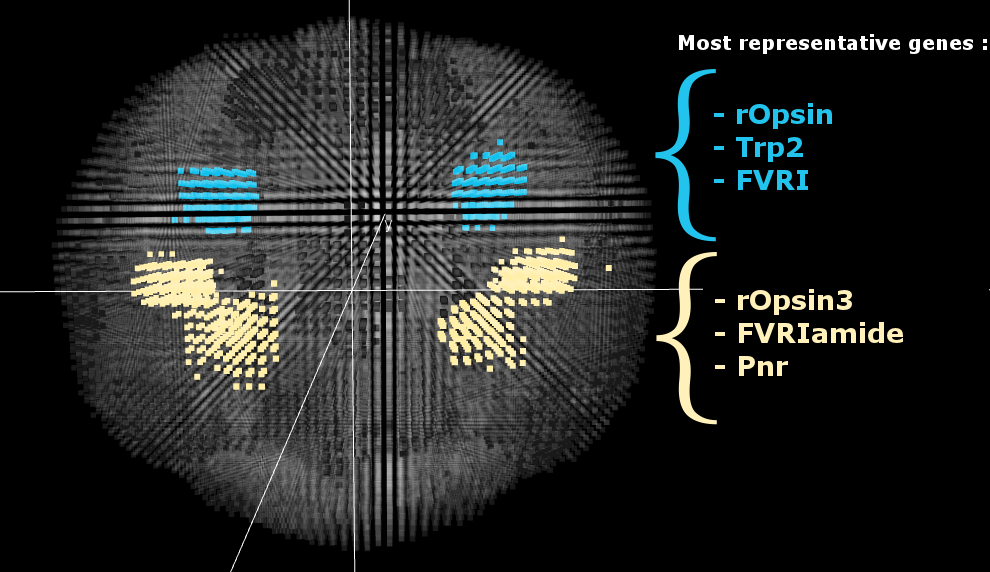
\includegraphics[width=1\linewidth]{gfx/chapter6/eyes.png}}
\caption{{\bf Eyes in the brain of Platynereis as clustered by the HMRF method.} Adult (blue cluster) and larval (yellow cluster) eyes in separate clusters with their top 3 most representative genes.}
\label{fig:valideyesclust}
	\end{figure}
	
	
	\begin{figure}[H]
\centerline{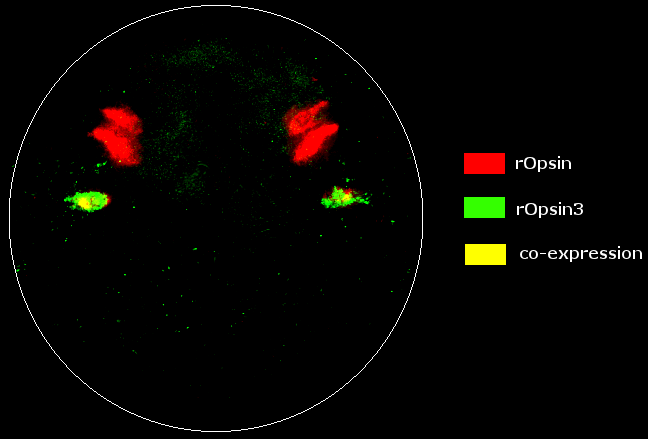
\includegraphics[width=1\linewidth]{gfx/chapter6/insitu.png}}
\caption{{\bf In-situ hybridization image for rOpsin and rOpsin3 in the full brain at 48hpf (Apical view).} Z-projection of the expression of rOpsin (red) in both the adult eyes and the larval eyes, rOpsin3 (green) specifically in the larval eyes and co-expression areas in some areas of the larval eyes in the full brain of {\it{Platynereis}} at 48hpf. The white circle is a schematic outline of the brain.  This image been obtained directly from the data obtained in \cite{Tomer10}.}
\label{fig:valideyesinsitu}
	\end{figure}
	
	
		\subsection{Mushroom bodies}
		As well as the eyes, a second region of the {\it{Platynereis}} brain, the mushroom bodies (which corresponds to the pallium, a layers of neurons that cover the upper surface of the cerebrum in vertebrates \cite{Tomer10}), are also clearly identified by our approach (Figure \ref{fig:validmush}). They have been described anatomically and molecularly in \platy{} in \cite{Tomer10}. In this paper the authors define the mushroom bodies as a ventral regions, define by a subset of the expression pattern of gene \emph{BF1} and by the same genes as the top scoring genes that define my cluster, \emph{Emx, Wnt8}. As shown schematically in Figure \ref{fig:validmushtom} from \cite{Tomer10}, the localization of the mushroom bodies (MB) is coherent with the inferred cluster in Figure \ref{fig:validmush}.
		
	\begin{figure}[H]
\centerline{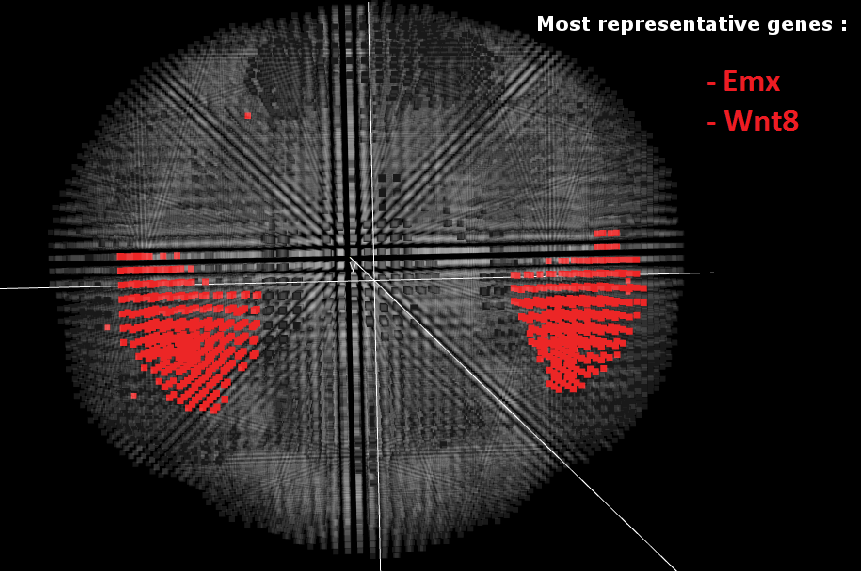
\includegraphics[width=0.8\linewidth]{gfx/chapter6/mush.png}}
\caption{{\bf Mushroom bodies in the brain of Platynereis as clustered by the HMRF method.} Mushroom bodies and their most representative genes.}
\label{fig:validmush}
	\end{figure}
	
	\begin{figure}[H]
\centerline{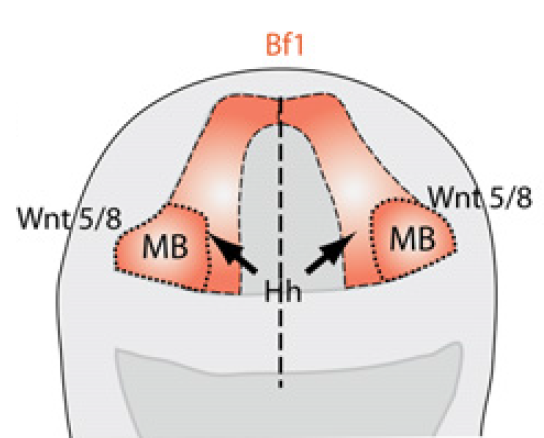
\includegraphics[width=0.6\linewidth]{gfx/chapter6/mush_tomer.png}}
\caption{{\bf Schematic representation of the mushroom bodies in the brain of Platynereis by \cite{Tomer10}.} MB: mushroom bodies}
\label{fig:validmushtom}
	\end{figure}
		\subsection{Motor regions}
		Experimentally, when the brain is dissociated from the rest of the larvae, the most basal part contains the developing motor regions. These motor regions are clustered together as shown in Figure \ref{fig:muscles}. Indeed, the green cluster defines a region on the basal side of the larvae that can be associated both by its localization and by its most representative genes ({\it{MyoD}} \cite{weintraub91,michelson90} and {\it{LDB3}} \cite{krcmery10,marziliano07}) with the starting point of the developing muscles of the adult animal. {\it{MyoD}} has been shown to play a key role in the differentiation of muscles during development in vertebrates and invertebrates \cite{weintraub91,michelson90} and {\it{LDB3}} codes for the protein LDB3, which interacts with the myozenin gene family that has been implicated in muscle development in vertebrates \cite{marziliano07}.\\
		
	\begin{figure}[h]
\centerline{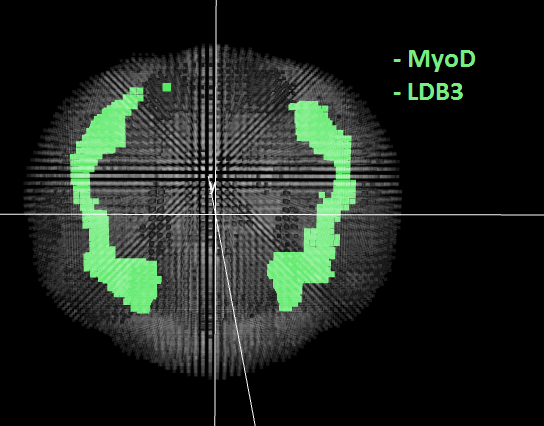
\includegraphics[width=0.8\linewidth]{gfx/chapter6/muscles.png}}
\caption{{\bf Developing motor region in the brain of Platynereis as clustered by the HMRF method.} Basal motor regions and their most representative genes.}
\label{fig:muscles}
	\end{figure}
		
		Again, it is possible to cross-validate the function of this region against previous studies. In this case, \cite{Fischer10} used muscle specific phalloidin staining at 48hpf to visualize the developing motor region in the larvae's brain, the result of which is reproduced from \cite{Fischer10} in Figure \ref{fig:muscles_stain}. 
		
		
	\begin{figure}[H]
\centerline{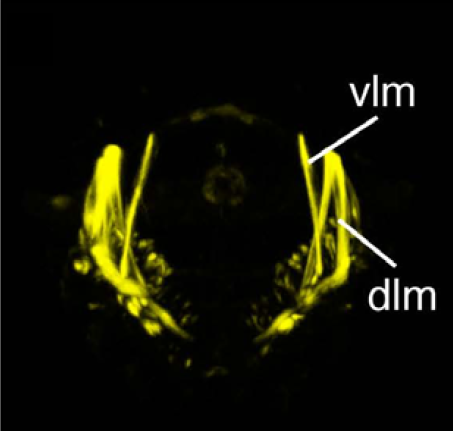
\includegraphics[width=0.6\linewidth]{gfx/chapter6/muscle_stain.png}}
\caption{{\bf Developing motor region in the brain of Platynereis visualized in-situ by phalloidin staining.} This Figure is reproduced from \cite{Fischer10}. vlm: ventral longitudinal muscle; dlm: dorsal longitudinal muscle.}
\label{fig:muscles_stain}
	\end{figure}
	
	The eyes, the mushroom bodies and the developing motor regions validation provided good confidence that the HMRF method yielded sensible results and that the gene scoring developed was able to successfully define a specific gene expression fingerprint for each cluster. However, of the $K=33$ clusters, some of the defined regions are not easily recognizable when compared against the known biology of \platy{}. These regions are very interesting as they may represent previously unstudied sub-populations of cells in the brain. 



	\section{Generating functional hypotheses about unknown biological tissues}
	As well as identifying clusters corresponding to known cell types, I also identified clusters that might correspond to less well studied subtypes with specific biological functions. \\
	
	\begin{figure}[H]
\centerline{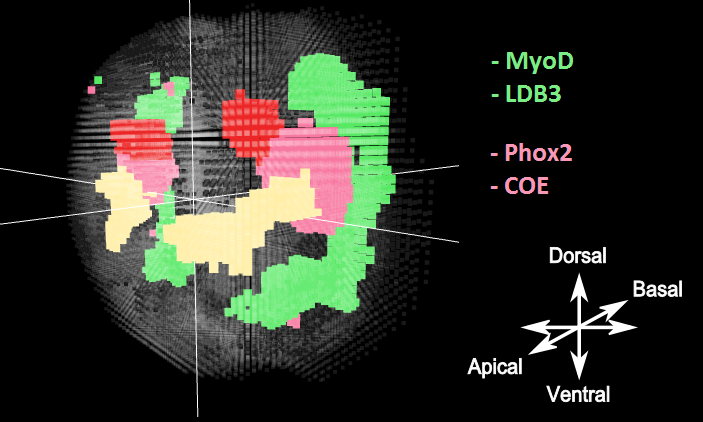
\includegraphics[width=0.8\linewidth]{gfx/chapter6/eyes_muscles.png}}
\caption{{\bf A putative tissue of developing neurons between the eyes and the larvae's developing muscles.} The yellow and red clusters are the eyes as seen in Figure \ref{fig:valideyesclust}. The green cluster represents the developing muscles on the basal side of the larvae, as the location and the most specific genes strongly suggest. The pink cluster is a putative tissue that makes an interesting link between the eyes and the muscles. The most representative gene of this tissue is Phox2, a homeodomain protein required for the generation of visceral motor-neurons in \emph{Drosophila} \cite{briscoe99}}
\label{fig:eyes_muscles}
	\end{figure}

	Given the location of the eyes (Figure \ref{fig:valideyesclust}) and the developing muscles (Figure \ref{fig:muscles}), the location of the pink cluster in Figure \ref{fig:eyes_muscles} is interesting. This cluster surrounds the larval eyes, the adult eyes and reaches the developing muscles described above. Looking at the most representative genes for this pink cluster, it is interesting to note the presence of {\it{Phox2}}, a homeodomain protein that has been shown to be necessary for the generation of visceral motor-neurons (neurons of the central nervous system that project their axons to directly or indirectly control muscles) as described generally in \cite{brunet02} and in \emph{Drosophila} \cite{briscoe99}. The second most representative gene, {\it{COE}}, has also been shown to play a role in \emph{Platynereis} and \emph{Drosophila} neural tissue development \cite{demilly11}. In this context, although we lack biological validation, we can hypothesise that the cells within this particular cluster could be developing neurons that link the eyes to the muscles of \emph{Platynereis}.\\
	
	 Although this hypothesis remains purely speculative and would need validation in the laboratory, this example is an interesting proof-of-concept that this clustering method can prove useful for hypothesis generation. Indeed, the analysis of the parameter values and the spatial localization attached to the clusters has allowed me to place with a reasonable level of confidence a functional hypothesis about a tissue that was not clearly defined either spatially or functionally. \\
	 
\section{Method sensitivity compared to other clustering methods}
	To complement the comparison work described in Chapter \ref{ch:simulations}, I decided to assess for the biological tissues outlined in the previous paragraphs the sensitivity of the HMRF method compared to the independent mixture model EM and to hClust.\\
	
	In Figure \ref{fig:hclust_clust} are shown the clusters obtained with the hClust method. Some of the regions are conserved across clustering techniques, in particular the eyes. however the hClsut results are much less precise than those of the HMRF method. In particular the both the adult and the larval eyes are clustered alongside a second region that has no biological meaning (red and yellow cluster in Figure \ref{fig:hclut_clust}). Furthermore, the developing muscles are not picked up at all by hClust.
	
	\begin{figure}[H]
\centerline{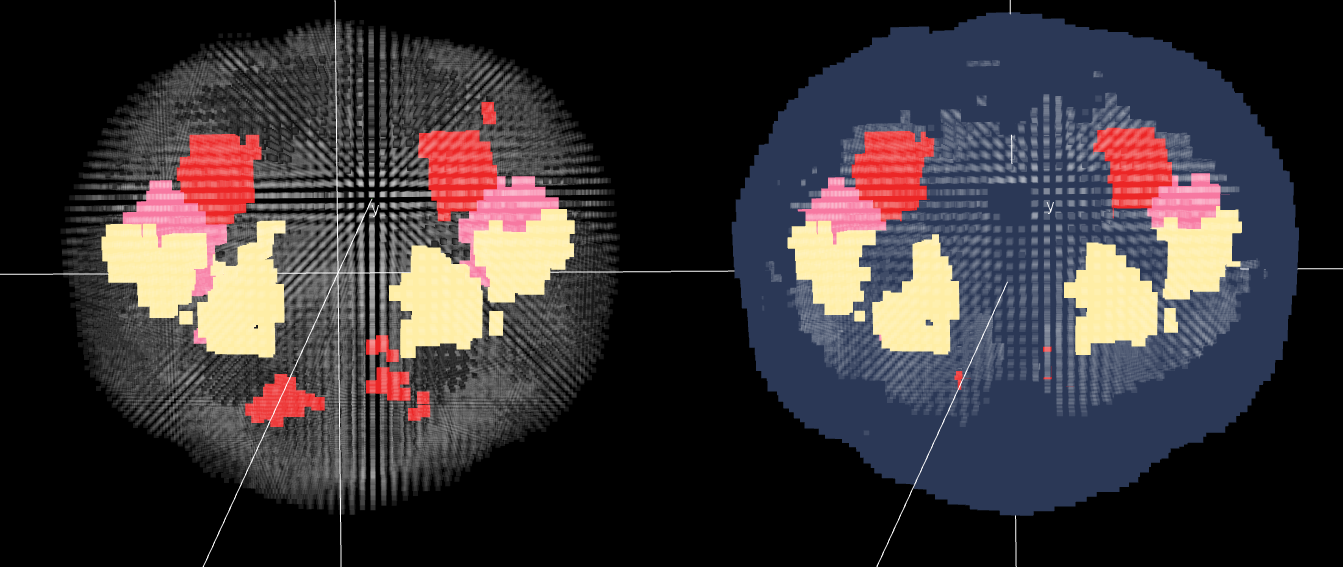
\includegraphics[width=\linewidth]{gfx/chapter6/hclust.png}}
\caption{Clusters obtained with hClust after alignment onto the MRF results. The Adult eyes are well isolated (red) although a region in the ventral part of the brain is classified in the same cluster which is biologically nonsensical. The larval eyes (yellow) are also picked up but along side a second region. Finally if hClust picks up a part of the putative tissue of developing neurones described above (pink), it does not find the muscles at all. Instead the region where the muscles are found by the HMRF method is part of a large cluster of cells forming a layer around the brain (purple cluster on the right).}
\label{fig:hclust_clust}
	\end{figure}
	
	In Figure \ref{fig:mixture_clust} are shown the clusters obtained with the independent mixture model method. It is generally close to the results obtained with the HMRF. However, the resulting picture is extremely noisy. Furthermore, for the muscles region, this noise is linked to biological imprecisions. Indeed, the developing muscles as shown biologically in figure \ref{fig:muscles_stain} do not present a either a dorsal or ventral region in the middle. 
	
	\begin{figure}[H]
\centerline{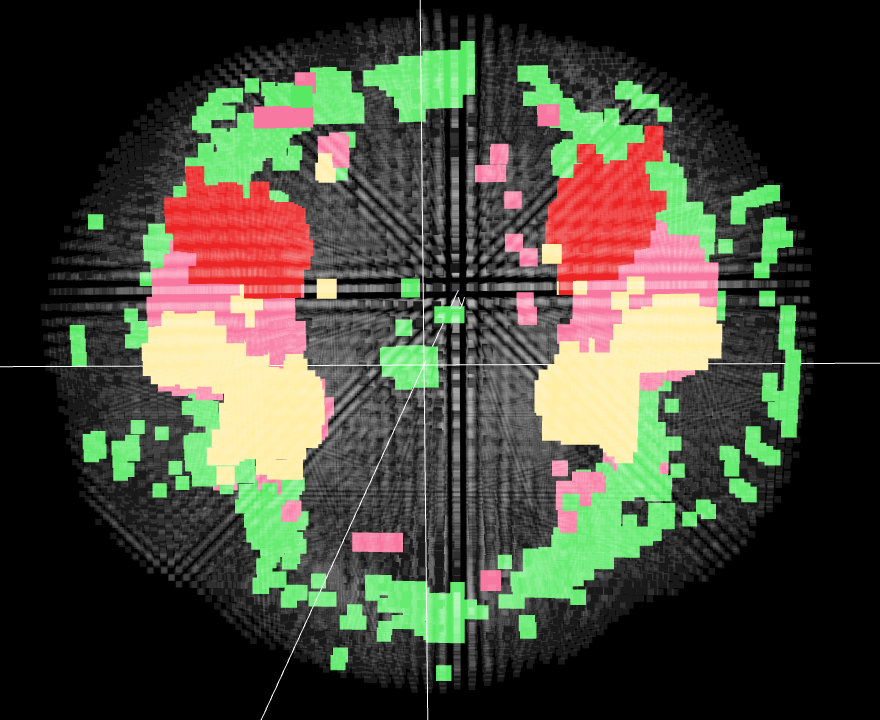
\includegraphics[width=\linewidth]{gfx/chapter6/mixture.png}}
\caption{Clusters obtained with the independent mixture model with the same initialization as the one used for the results presented in the paragraphs above for the HMRF. The Adult eyes are well isolated (red). The larval eyes (yellow) as well. The muscles and the region of potential developing neurons are picked up as well. However if all the regions are recognizable, they are extremely poorly defined spatially with a lot of noise and little spatial coherency. In the case of the muscles, when comparing with the in-situ imaging in Figure \ref{fig:muscles_stain}, it is clear that the HMRF results are closer to the biological reality as there is no fully dorsal or ventral regions in the developing muscles.}
\label{fig:mixture_clust}
	\end{figure}
	
	
	 

\section{Summary}
	
I applied the HMRF clustering method described in Chapter \ref{ch:HMRF} to the binarized in-situ hybridization data presented in Chapter \ref{ch:singlecell}. I described how the BIC method was adapted to chose the optimal number of clusters $K = 33$.\\

In order to analyse the resulting clusters, I developed a scoring method based on a ``specificity'' matrix which extracts the most specific genes for each cluster. Thanks to the 3D visualization tool described in Chapter \ref{ch:non_spatial_clustering_visualization}, and the most specifically expressed genes for each cluster, I was able to validate the method biologically by localizing 3 well studied regions of the brain. Additionally I checked that the top 3 genes were consistent with the known biology of \platy{}.\\

Furthermore, I demonstrated how my approach allows the generation of functional hypothesis about regions that are not well known. In particular, I discussed a previously unstudied tissue that may consist of developing neurons directly linking the eyes to the developing muscles.

%*****************************************
%*****************************************
%*****************************************
%*****************************************
%*****************************************
